\chapter{Måling på indgangsvælger}
\label{maalejournal_indgangsvaelger}

Denne målerapport dokumenterer målinger foretaget på projektets indgangsvaelger, opbygget som beskrevet i kapitel \ref{forforstaerker}. Målingen er foretaget på Fredrik Bajers Vej 7 i lokale B1-104 på Aalborg Universitet den 14. december 2010 af gruppe 311.

\subsection*{Formål}
\label{maalejournal_formaal}
Målingens formål er at:
\begin{itemize}
\item Kontrollere funktionen af indgangsvælgeren og finde evt. fejl
\item Måle dæmpningen for en tændt samt en slukket indgang i indgangsvælgeren.
\item Måle outputtet i forhold til hvor mange indgange der er valgt .
\item Måle indgangsimpedansen for indgangene, tændt og slukket.
\item Måle at frekvensgangen ved 20 Hz - 20 kHz 
\end{itemize}

\subsection*{Testobjekt}
\label{maalejournal_testobjekt}
Der vil i denne målerapport blive udført tests af indgangsvælgeren. Indgangsimpedansen måles for alle indgangene: De to stereo indgange og mikrofon indgangen. Alle indgangsimpedanserne måles for både en tændt og en slukket indgang.
Til frekvensmåling 
\begin{figure}[h]
\centering
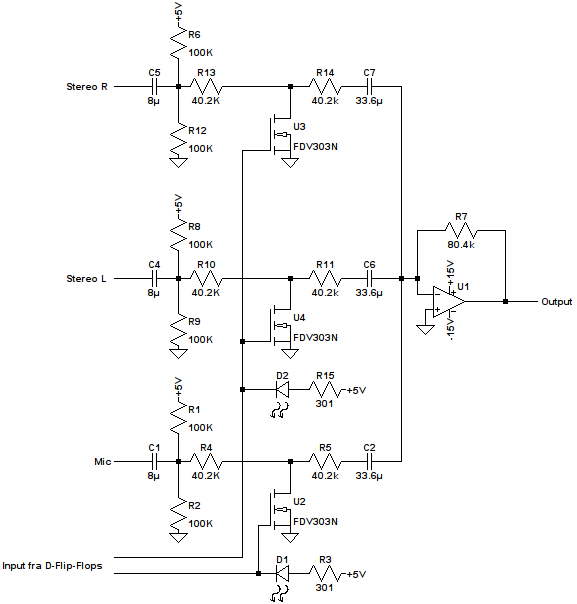
\includegraphics[scale=0.8]{maalerapporter/indgangsvaelger/indgangvaelger_ltspice_diagram.png}
\caption{Diagram over kredsløbet der testes.}
\label{maalerap-diagram_simulering}
\end{figure}

\subsection*{Teori}
\label{maalejournal_teori}
Teorien bag en impedansmåling, er at der skabes en spændingsdeling mellem en kendt reference modstand og indgangsmodstanden i det testede. Forholdet af spændingerne som ligger over modstandene svarer til forholdet mellem modstandene.

\subsection*{Måleopstilling}
\label{maalejournal_maaleopstilling}
Måleopstillingerne er vist på figur \ref{fig:indgang:maaleop-thd} .

\begin{figure}[h]
\centering
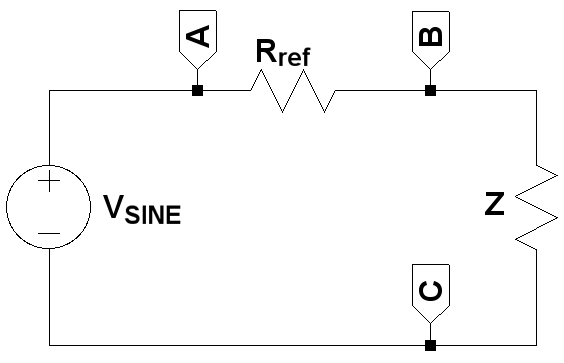
\includegraphics[scale=0.4]{maalerapporter/indgangsvaelger/impedansopstilling-forforstaerker.png}
\caption{Måleopstilling for impedansmåling}
\label{fig:indgang:maaleop-imp}
\end{figure}

\begin{figure}[h]
\centering
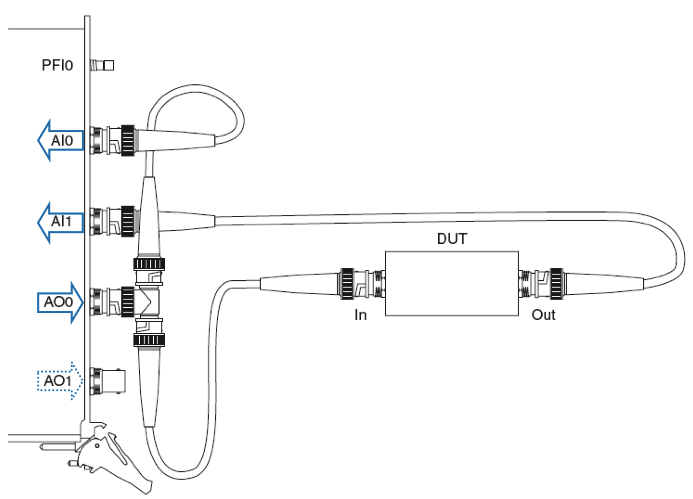
\includegraphics[scale=0.4]{maalerapporter/indgangsvaelger/maaleopstilling-thd-forforstaerker.png}
\caption{Måleopstilling for forstærkning-, frekvensgang- og forvrængningsmåling \cite{maaling-mm5}}
\label{fig:indgang:maaleop-thd}
\end{figure}

\subsection*{Anvendt udstyr}
\label{indgang:maalejournal_anvendtudstyr}

\begin{table}[h]
\centering
\begin{tabular}{l|c|l}
\hline\hline
Instrument & AAU-nr. & Fabrikant, type m.v. \\
\hline\hline
Oscilloskop & 33866 & Agilent 54621A \\[4pt]
Oscillator & 07995 & B\&O RC-oscillator TG7 \\[4pt]
Spændingsforsyning & 39897 & HAMEG HM7042 \\[4pt]
Spændingsforsyning & 33901 & HAMEG HM7042 \\[4pt]
Multimeter & 33048 & Fluke and Philips FLUKE 37 \\[4pt]
Multimeter & 08518 & Fluke and Philips FLUKE 37 \\[4pt]
Audioanalysator & 76986 & National Instruments NI-PCI-4461 \\
\hline\hline
\end{tabular}
\label{tab:indgang:maaleudstyr_forforstaerker}
\end{table}

\subsection*{Måleprocedure}
\label{indgang:maalejournal_maaleprocedure}
Proceduren for impedansmålingen er:

\begin{enumerate}
\item Generatoren, kaldet $V_\mathrm{SINE}$ på figur \ref{fig:indgang:maaleop-imp}, indstilles til en effektivspænding på 21,1 mV (indstilles med oscilloskop) ved 1 kHz og tilsluttes
\item Reference modstanden, kaldet $R_\mathrm{ref}$ på figur \ref{fig:indgang:maaleop-imp}, vælges til 10 k\ohm~ og tilsluttes
\item Spændingsfaldet fra terminal A til terminal B, som på figur \ref{fig:fig:indgang:maaleop-imp}, måles
\item Spændingsfaldet fra terminal B til terminal C, som på figur \ref{fig:fig:indgang:maaleop-imp}, måles
\end{enumerate}
Herefter slukkes for indgang, og målingen foretages igen. Dette gentages for hver indgang.

Proceduren for forstærkning-, frekvensgang- og forvrængningsmålingen er:

\begin{enumerate}
\item En spændingsforsyning indstilles til $\pm15~V$ (indstilles med multimeteret) og tilsluttes.
\item En spændingsforsyning indstilles til 5 V (indstilles med multimeteret) og tilsluttes.
\item Testobjektet tilsluttes som på figur \ref{fig:indgang:maaleop-thd}
\item Kanalen der måles på, indstilles ved hjælp af trykknappen.
\item Programmet $"$Swept Sine - Linear Response and Harmonic Distortion (DAQmx)$"$ startes
\item $"$Start frequency$"$ under Source settings sættes til 20 Hz
\item $"$Stop frequency$"$ under Source settings sættes til 20 kHz
\item $"$Amplitude$"$ under Source settings sættes til 2 V
\item $"$THD units$"$ sættes til \%
\item $"$AI Range$"$ for Stimulus channel sættes til $\pm$ 0,316 V\fixme{Check}
\item $"$AI Range$"$ for Respons channel sættes til $\pm$ 3,16 V\fixme{dem her}
\item $"$Sampling frequency$"$ sættes til 204,8 kHz
\end{enumerate}

Samme procedure gennemføres, hvor amplituden i punkt 7 i stedet sættes til 200 mV. Dermed opnåes resultater for både maksimums- og minimumsinput. 

\subsection*{Resultater}
\label{maalejournal_resultater}

Impedansmålingen gav effektivspændingerne vist i tabel \ref{tab:resultatimpedans_indgang}. Disse spændinger bruges til at regne testobjektets indgangsimpedans, med formel (\ref{equ:zresultat-indgang}) \cite{maaling-mm4}.%\fixme{kilde: Ole Kiel Jensen, mm4 Maaleteknik}.

\begin{equation}
\label{equ:zresultat-indgang}
\vert Z \vert = \frac{\vert V_Z \vert}{\vert V_{R_\mathrm{ref}} \vert} \cdot R_\mathrm{ref}
\end{equation} 

\begin{table}[h]
\centering
\begin{tabular}{l|c|c|l}

\hline\hline
\multicolumn{4}{c}{\textbf{Mikrofon Indgang}} \\
\hline\hline
& Målt værdi & Beregnet værdi & Enhed \\
\hline\hline
Tændt: $V_{R_\mathrm{ref}}$ & 5,1& & mV effektiv\\[4pt]
Tændt: $V_Z$ & 16,1 & & mV effektiv\\[4pt]
Tændt: $R_\mathrm{i,forforstaerker}$ & & 31,56 & k\ohm \\
Slukket: $V_{R_\mathrm{ref}}$ & 6,5& & mV effektiv\\[4pt]
Slukket: $V_Z$ & 14,7 & & mV effektiv\\[4pt]
Slukket: $R_\mathrm{i,forforstaerker}$ & & 22,62 & k\ohm \\
\hline\hline
\multicolumn{4}{c}{} \\
\hline\hline
\multicolumn{4}{c}{\textbf{Stereo L}} \\
\hline\hline
& Målt værdi & Beregnet værdi & Enhed \\
\hline\hline
Tændt: $V_{R_\mathrm{ref}}$ & 5,1& & mV effektiv\\[4pt]
Tændt: $V_Z$ & 16,1 & & mV effektiv\\[4pt]
Tændt: $R_\mathrm{i,forforstaerker}$ & & 31,56 & k\ohm \\
Slukket: $V_{R_\mathrm{ref}}$ & 6,5& & mV effektiv\\[4pt]
Slukket: $V_Z$ & 14,7 & & mV effektiv\\[4pt]
Slukket: $R_\mathrm{i,forforstaerker}$ & & 22,62 & k\ohm \\
\hline\hline
\multicolumn{4}{c}{} \\
\hline\hline
\multicolumn{4}{c}{\textbf{Stereo R}} \\
\hline\hline
& Målt værdi & Beregnet værdi & Enhed \\
\hline\hline
Tændt: $V_{R_\mathrm{ref}}$ & 5,1& & mV effektiv\\[4pt]
Tændt: $V_Z$ & 16,1 & & mV effektiv\\[4pt]
Tændt: $R_\mathrm{i,forforstaerker}$ & & 31,56 & k\ohm \\
Slukket: $V_{R_\mathrm{ref}}$ & 6,5& & mV effektiv\\[4pt]
Slukket: $V_Z$ & 14,7 & & mV effektiv\\[4pt]
Slukket: $R_\mathrm{i,forforstaerker}$ & & 22,62 & k\ohm \\
\hline\hline
\end{tabular}
\caption{Resultater af impedansmåling}
\label{tab:resultatimpedans_indgang}
\end{table}

Frekvensgangen og THD blev målt for de forskellige indgange. Resultaterne er vist i figur \ref{fig:apind:frek200mv} til figur \ref{fig:apind:thd2vslukket}. Resten af resultaterne kan findes på CD'en\fixme{henvisning}. Spændingsniveauer angivet i V og mV er amplitude værdier. 


\begin{figure}[h]
\centering
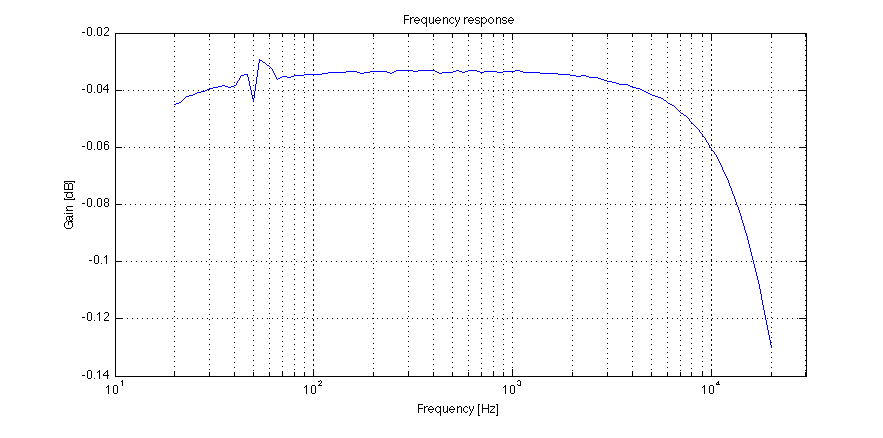
\includegraphics[width=\textwidth]{maalerapporter/indgangsvaelger/Indgangsvlger-mic-200mv-frek.png}
\caption{Frekvensgangen for mikrofonindgangen på indgangsvælgeren ved 200 mV.}
\label{fig:apind:frek200mv}
\end{figure}


\begin{figure}[h]
\centering
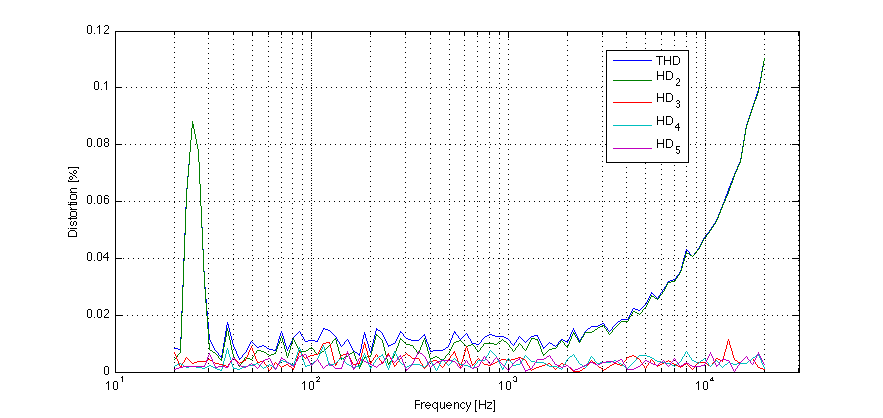
\includegraphics[width=\textwidth]{maalerapporter/indgangsvaelger/Indgangsvlger-mic-200mv-thd.png}
\caption{THD for mikrofonindgangen på indgangsvælgeren ved 200 mV.}
\label{fig:apind:thd200mv}
\end{figure}


\begin{figure}[h]
\centering
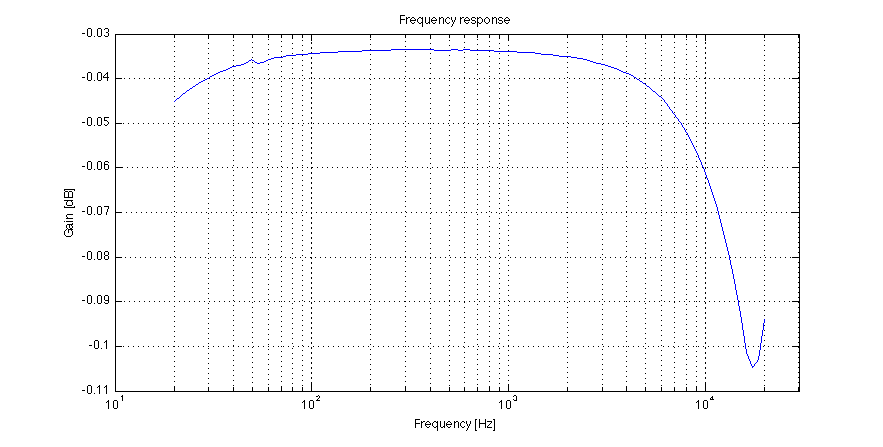
\includegraphics[width=\textwidth]{maalerapporter/indgangsvaelger/Indgangsvlger-mic-2v-frek.png}
\caption{Frekvensgangen for mikrofonindgangen på indgangsvælgeren ved 2V.}
\label{fig:apind:frek2v}
\end{figure}


\begin{figure}[h]
\centering
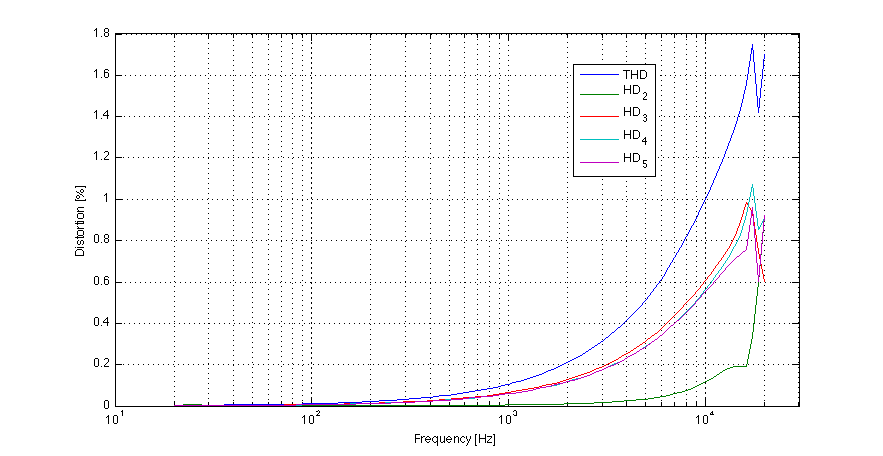
\includegraphics[width=\textwidth]{maalerapporter/indgangsvaelger/Indgangsvlger-mic-2v-thd.png}
\caption{THD for mikrofonindgangen på indgangsvælgeren ved 2 V.}
\label{fig:apind:thd2v}
\end{figure}


\begin{figure}[h]
\centering
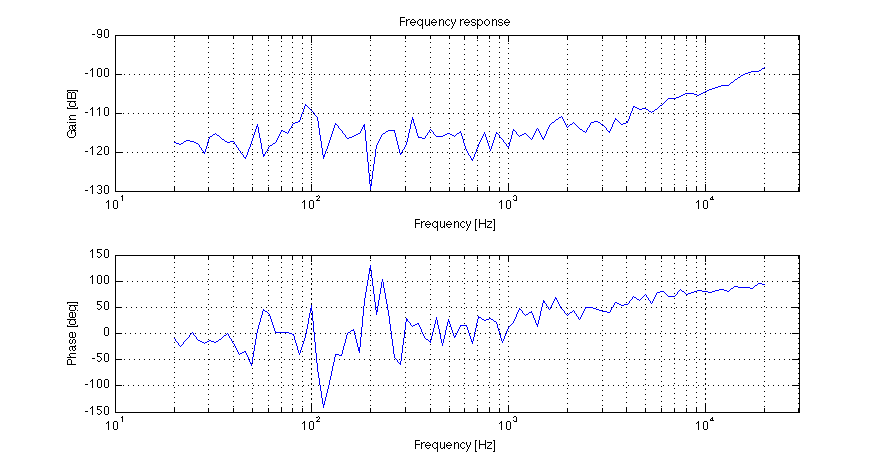
\includegraphics[width=\textwidth]{maalerapporter/indgangsvaelger/Indgangsvlger-mic-2v-slukket-frek.png}
\caption{Frekvensgangen og fasedrejet for mikrofonindgangen for et slukket signal, på indgangsvælgeren ved 2V.}
\label{fig:apind:frek2vslukket}
\end{figure}


\begin{figure}[h]
\centering
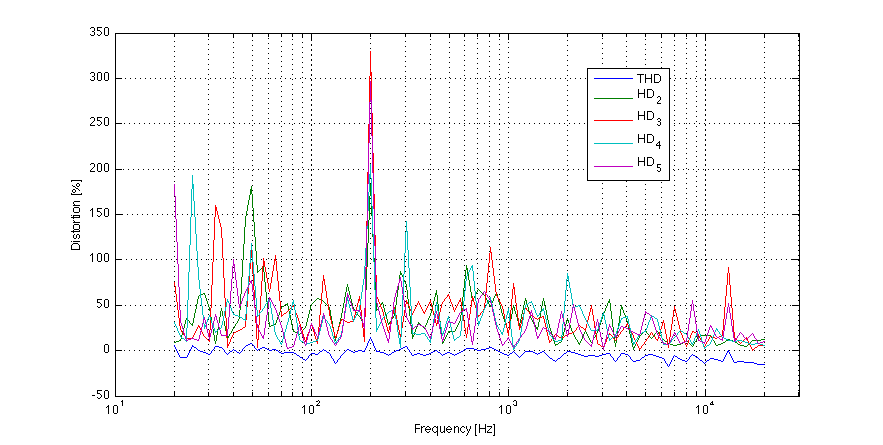
\includegraphics[width=\textwidth]{maalerapporter/indgangsvaelger/Indgangsvlger-mic-2v-slukket-thd.png}
\caption{THD for mikrofonindgangen for et slukket signal, på indgangsvælgeren ved 2 V.}
\label{fig:apind:thd2vslukket}
\end{figure}

\subsection*{Måleusikkerheder}
\label{maalejournal_maaleusikkerheder}
De væsentligste usikkerheder er:
\begin{itemize}
\item Komponent tolerancer
\item Påvirkning fra måleinstrument
\item Måleinstrument unøjagtighed
\item Støj, 50 Hz brum
\item Anden indstråling
\end{itemize}